% final draft

\chapter{Literatur zum Themengebiet Articulation Work} % (fold)
\label{cha:literatur_zum_themengebiet_articulation_work}

Dieser Anhang stellt die Literatur zu „Articulation Work“ umfassend dar. Er dient als Ergänzung zu den in Kapitel \ref{cha:articulation_work} eingeführten Konzepten und Inhalten. Insbesondere wurden die hier beschriebenen Arbeiten hinsichtlich ihrer Relevanz für die Begriffsbestimmung zu „Articulation Work“ und deren Unterstützung beurteilt. Die als relevant identifizierten Arbeiten wurden in den Abschnitten \ref{sec:aw_begriffsbestimmung}, \ref{sec:arten_von_articulation_work} und \ref{sec:unterstützung_von_articulation_work} umfassender dargestellt.

\section{Literaturquellen} % (fold)
\label{sec:literaturquellen}

In der Literatursuche wurden Datenbanken aus den Bereichen Informatik, Psychologie, Soziologie, den Wirtschaftswissenschaften sowie der Organisationslehre durchsucht. Nach der initialen Suche wurde jeweils auch die in den gefundenen Arbeiten referenzierte Sekundärliteratur aufgearbeitet. Des weiteren wurden mit Hilfe von rückwärts verlinkenden Datenbanken (wo vorhanden) Publikationen erfasst, die auf die bislang gefundenen Arbeiten referenzieren. Die so identifizierten Publikationen wurden ebenfalls hinsichtlich ihrer Relevanz überprüft.

Die in der Suche berücksichtigten Datenbanken bzw. Meta-Suchmaschinen sind:
\begin{description}
	\item[Domänenspezifische Datenbanken]\ 
		\begin{itemize}
			\item INSPEC\footnote{via http://ovidsp.ovid.com} (Naturwissenschaften)
			\item Business Source Premier\footnote{via http://search.ebscohost.com/} (Wirtschaftswissenschaften)
			\item PsycINFO\footnote{via http://ovidsp.ovid.com} (Psychologie)
			\item PSYNDEXplus\footnote{via http://ovidsp.ovid.com} (Psychologie)
			\item SocINDEX\footnote{via http://search.ebscohost.com/} (Soziologie)
			\item ERIC\footnote{http://www.eric.ed.gov/} (Pädagogik)
			\item ACM Guide\footnote{http://portal.acm.org/guide.cfm} (Informatik)
		\end{itemize}
	\item[Verlags-Datenbanken]\ 
		\begin{itemize}
			\item ACM Digital Library\footnote{http://portal.acm.org/dl.cfm} (Informatik)
			\item IEEE XPlore\footnote{http://ieeexplore.ieee.org} (Informatik)
			\item SpringerLink\footnote{http://www.springerlink.de} (fächerübergreifend)
			\item ScienceDirect\footnote{http://www.sciencedirect.com} (fächerübergreifend)
			\item Emerald\footnote{http://www.emeraldinsight.com} (Wirtschaftswissenschaften)
			\item Wiley Interscience\footnote{http://www3.interscience.wiley.com} (fächerübergreifend)
		\end{itemize}
	\item[Meta-Suchmaschinen]\ 
	 	\begin{itemize}
	 		\item Google Scholar\footnote{http://scholar.google.com/} (fächerübergreifend)
	 		\item CiteSeerX\footnote{http://citeseerx.ist.psu.edu/} (Naturwissenschaften und Informatik)
	 	\end{itemize}
\end{description}

% section literaturquellen (end)

\section{Relevante Literatur} % (fold)
\label{sec:relevante_literatur}

Die im Folgenden genannten Arbeiten beziehen sich in unterschiedlicher Weise auf das Themengebiet „Articulation Work“. Es konnten vier Kategorien von Arbeiten identifiziert werden, die sich hinsichtlich ihres inhaltlichen Fokus unterscheiden:
\begin{enumerate}[(I)]
	\item Arbeiten, die sich mit der grundlegenden Konzeption von „Articulation Work“ beschäftigen und keine Aussage zu deren Unterstützung machen.
	\item Arbeiten, in denen „Articulation Work“ als erklärendes Rahmenwerk für beobachtete Phänomene verwendet wird, und in der Folge das Hauptaugenmerk auf diese Phänomene gelegt wird, ohne nochmals näher auf „Articulation Work“ einzugehen.
	\item Arbeiten, die auf die Unterstützung von Articulation Work eingehen.
	\item Arbeiten, in denen „Articulation Work“ lediglich erwähnt wird, allerdings nicht näher darauf Bezug genommen wird.
\end{enumerate}

In chronologischer Reihenfolge des Erscheinens sind die folgenden Arbeiten einer oder mehreren der genannten Kategorien zuzuordnen (Kategorie jeweils in Klammer angeführt):

\begin{description}
	\item[\citet{Strauss85}] (I) prägt in dieser Arbeit den Begriff „Articulation Work“ und beschreibt dieses auf konzeptioneller Ebene ohne eine unmittelbaren Praxis- bzw. Umsetzungsbezug herzustellen.
	\item[\citet{Gasser86}] (I) beschreibt die Integration von Computerunterstützung in alltägliche Arbeitsabläufe und die Anpassungsleistung der arbeitenden Individuen, wenn die aktuelle Arbeitssituation nicht mehr mit dem der Computerunterstützung zugrunde liegenden Modell übereinstimmt. Er identifiziert dabei spezifische Aktivitäten, die im Rahmen der ablaufenden „Articulation Work“ auftreten können.
	\item[\citet{Gerson86}] (I, II) zeigen die konkrete Manifestation von Articulation Work in einer Fallstudie aus einem Versicherungskonzern und identifizieren daraus die organisationalen Rahmenbedingungen, die zu jenen Problemen führen, die „Articulation Work“ notwendig machen.
	\item[\citet{Bendifallah87}] (II) untersuchen bezugnehmend auf \citet{Gasser86} „Articulation Work“ im Kontext von IT-Support-Arbeit in Unternehmen anhand von zwei Fallstudien und identifizieren dabei zwei unterschiedliche Strategien bei der Durchführung derselben. Im Detail gehen sie jedoch nicht auf die konkret zu setzenden Maßnahmen ein.
	\item[\citet{Fujimura87}] (I) leitet die grundlegende Unterscheidung zwischen „Production Work“ und „Articulation Work“ anhand einer Fallstudie aus dem wissen\-schaftlich-medizinischen Forschungsbetrieb ab. Sie bleibt dabei auf konzeptueller Ebene und beschreibt die auftretenden Phänomene, geht jedoch nicht auf unterstützende Maßnahmen ein.
	\item[\citet{Strauss88}] (I) detailliert und erweitert seine Konzepte und setzt diese in den Kontext organisationaler Projektarbeit (im dort beschrieben Verständnis im Wesentlichen identisch mit „non-routine collective activity“). Anhand einer Fallstudie aus dem Krankenhaus-Organisations-Bereich zeigt er das Auftreten von „Articulation Work“ in der Praxis, beschäftigt sich jedoch nicht mit möglicherweise unterstützenden Interventionen.
	\item[\citet{Schmidt90}] (I) beschreibt ein Framework für die Analyse kooperativer Arbeit und erwähnt dabei „Articulation Work“ als ein zu berücksichtigendes Konzept. Diese Arbeit bildet die Grundlage für die im Hinblick auf die Unterstützung von „Articulation Work“ relevantere Arbeit von \citet{Schmidt92}.
	\item[\citet{Mi91}] (III) betrachten „Articulation Work“ im Kontext der Softwareentwicklung und argumentieren für deren explizite Berücksichtigung in Software Engineering Prozessen. Sie schlagen einen formalisierten Prozess zur Durchführung von „Articulation Work“ vor und führen einen Satz von regelbasierten Heuristiken zur konkreten Durchführung ein. Sie sind damit die ersten, die sich explizit mit der Unterstützung von „Articulation Work“ beschäftigen.
	\item[\citet{Schmidt92}] (I, III) begründen mit dieser Arbeit eine Entwicklungsrichtung der \gls{CSCW}, die neben der Unterstützung der eigentlichen produktiven Arbeit auch auf die Unterstützung von „Articulation Work“ fokussiert. Sie beschreiben damit erstmals Anforderungen an die technische Unterstützung von „Articulation Work“ und Möglichkeiten zu deren Umsetzung.
	\item[\citet{Bannon93}] (II) zeigen in diesem Sammelwerk die ersten Ergebnisse des COMIC-Projektes \citep{Rodden95} und erwähnen dabei in einzelnen Beiträgen „Articulation Work“ als ein im Bereich der \gls{CSCW} zu berücksichtigendes Konzept.
	\item[\citet{Corbin93}] (I) beschäftigen sich mit der Festlegung von Interaktionsmodalitäten in kooperativer Arbeit durch „Articulation Work“ und detaillieren dabei das Verständnis von expliziter „Articulation Work“, indem sie mögliche Zeitpunkte des Auftretens sowie Schritte bei deren Durchführung nennen.
	\item[\citet{Strauss93}] (I) fasst im Rahmen einer umfassenderen Arbeit zur Entwicklung einer „Theory of Action“ seine Überlegungen zur Rolle und Ausgestaltung von „Articulation Work“ zusammen und würdigt diese kritisch. Konkrete Maßnahmen zur Unterstützung oder Ermöglichung von Articulation Work sind aber auch hier nicht vorhanden.
	\item[\citet{Bowers94}] (III) ist Editor eines COMIC-Deliverables \citep{Rodden95}, in dem zum ersten Mal auf die in \citep{Schmidt96} ausformulierten Anforderungen zur technischen Unterstützung von „Articulation Work“ eingegangen wird.
	\item[\citet{Lenoir94}] (IV) erwähnt „Articulation Work“ (konkret die Arbeit von \citet{Fujimura87}) als Beispiel der Verknüpfung unterschiedlicher wissenschaftlicher Arbeitskontexte, geht aber dann nicht näher auf „Articulation Work“ ein.
	\item[\citet{Schmidt94}] (III) rephrasiert im Wesentlichen \citep{Schmidt90} mit Fokus auf den Aspekt der kooperativen Arbeit (und nicht der Computerunterstützung derselben). Er detailliert darin die Artikulationsnotwendigkeiten bei kooperativer Arbeit, führt jedoch hinsichtlich der Unterstützung von Articulation Work keine zusätzlichen Anforderungen ein.
	\item[\citet{Schmidt95}] (III) basiert wie \citep{Schmidt94} auf \citep{Schmidt90}, leitet jedoch inhaltlich bereits zu der oben im Detail behandelten Arbeit von \citet{Schmidt96} über.
	\item[\citet{Grinter95}] (II) beschreibt die Verwendung von Konfigurations-Management-Systemen zur Koordination von Softwareentwicklungs-Prozessen. Sie bezieht sich dabei am Rand auf „Articulation Work“ (via \citep{Schmidt92}), führt diesen Aspekt aber nicht näher aus. Diese Arbeit bildet jedoch die Grundlage für die hinsichtlich der Unterstützung von „Articulation Work“ relevantere Arbeit derselben Autorin \citep{Grinter96}.
	\item[\citet{Simone95}] (III) konkretisieren die in \citet{Schmidt96} beschriebene Notation zur Spezifikation von Koordinationsmechanismen in \gls{CSCW}-Systemen und bereiten damit den Weg zur technischen Unterstützung von „coordinating predefined work“, die in \citep{Divitini00} umfassend beschrieben ist.
	\item[\citet{Grinter96}] (III) betrachtet die Rolle von „Articulation Work“ im Kontext der Softwareentwicklung und zeigt anhand zweier qualitativer empirischer Studien die Auswirkungen eines computerbasierten Configuration Management Systems bei der kooperativen Erstellung von Software.
	\item[\citet{Schmidt96}] (I, III) entwickeln in ihrer Arbeit ein generisches Vorgehen zur Konzeption von technischer Unterstützung von „Articulation Work“. Aufbauend auf früheren Arbeiten der Autoren (z.B. \citep{Schmidt90} und \citep{Schmidt92}) formulieren die Autoren eine Notation zur Spezifikation von \gls{CSCW}-Systemen, die auf der Unterstützung von „Articulation Work“ aufbauen.
	\item[\citet{Bannon97}] (II) beschreiben die Verwendung von „Common Information Spaces“ im Kontext von \gls{CSCW} und identifizieren die Artikulations-Bedürfnisse, die im Rahmen der Verwendung derselben auftreten können. Die Autoren gehen nicht näher auf die Umsetzung oder Unterstützung dieser konkreten Ausprägungen von „Articulation Work“ ein.
	\item[\citet{Fjuk97}] (I, III) versuchen die Konzepte von „Articulation Work“ durch eine Abbildung auf die Konzepte der „Activity Theory“ zu konkretisieren. Die Autoren geben dabei neben der Erweiterung der konzeptionellen Grundlagen auch mögliche Ansatzpunkte für die Unterstützung durch rechnerbasierte Werkzeuge an.
	\item[\citet{Fjuk97a}] (II) verwendet die Ansätze von \citet{Strauss93}, um die Interaktion in computerbasierten kooperativen Lernumgebungen (also in \gls{CSCL}-Systemen) zu betrachten. Sie verwendet dabei „Articulation Work“ als Analysedimension (als jener Teil des Arbeitsablaufs, in dem Interaktion zwischen den Lernenden vorrangig auftritt), gehen jedoch nicht näher auf deren Unterstützung ein.
	\item[\citet{Simone97}] (IV) beschreiben ein System zur Generierung von Awareness in kooperativen Anwendungen und erwähnen dabei am Rande „Articulation Work“, als einen Aspekt, bei dessen Unterstützung das System interessant sein könnte.
	\item[\citet{Simone97a}] (III) berichten über den aktuellen Stand der Entwicklung bei der technischen Unterstützung von Koordinationsmechanismen in CSCW-Systemen. Sämtliche hier enthaltenen Ergebnisse werden umfassender in \citep{Divitini00} dargestellt.
	\item[\citet{Kling98}] (II) beschreiben „Articulation Work“ als einen Aspekt, dessen Unterstützung bei der Gestaltung von „human centered (computer) systems“ zu berücksichtigen ist. Sie gehen jedoch nicht unmittelbar auf die mögliche Form der Unterstützung ein.
	\item[\citet{Carstensen99}] (III) führen Aspekte von \citep{Schmidt96} genauer oder aus einem anderen Betrachtungswinkel aus, fügen aber dem Verständnis von „Articulation Work“ bzw. deren Unterstützung keine neuen Aspekte hinzu.
	\item[\citet{Schmidt99}] (III) betonen basierend auf \citep{Schmidt96} den dynamischen Charakter von „Articulation Work“, die in einem Arbeitsablauf je nach Kontext unterschiedliche Ausprägungen annehmen kann. Sie fordern eine Berücksichtigung dieser Dynamik in technischen Werkzeugen zur Unterstützung von „Articulation Work“, fügen aber den Ausführungen von \citep{Schmidt96} keine fundamental neuen Anforderungen hinzu. Die Autoren leiten mit dieser Arbeit über zu der erstmals in \citet{Simone99} vorgestellten technischen Implementierung des in den vorgegangenen Publikationen konzipierten Werkzeugs.
	\item[\citet{Simone99}] (III) stellen als Umsetzung der in \citep{Schmidt96} aufgestellten Forderungen zur Unterstützung von „Articulation Work“ durch \gls{CSCW}-Systeme den „Reconciler“ vor, ein auf auf Java und \gls{CORBA} basierendes Software-Modul, dass den globalen Kontext und Zustand eines (digitalen) Arbeitsobjektes bei dessen Bearbeitung durch ein Individuum offenlegt und dadurch die Entwicklung einer gemeinsamen Sicht auf geteilt benutzte Objekte ermöglicht und die Vermeidung von Konflikten unterstützt. Der „Reconciler“ ist damit ein technisches Werkzeug zur Unterstützung von „situated Articulation Work“, die Arbeit detailliert jedoch lediglich die in \citep{Schmidt96} genannten Unterstützungsaspekte um diese technisch implementierbar zu machen.
	\item[\citet{Suchman99}] (II) beschäftigt sich mit „invisible work“ in denen Arbeitsartefakte an die tatsächlichen Erfordernisse des jeweiligen Arbeitskontext angepasst werden („design-for-use“). Sie argumentiert für die Anerkennung (also Sichtbarmachung) dieser Arbeit durch die Entwicklung expliziter Design-Praktiken, geht aber nicht näher auf deren Ausgestaltung ein.
	\item[\citet{Star99}] (III) verfassen die einzige Arbeit, in der Strauss selbst Stellung zur Unterstützung von „Articulation Work“ im Generellen und der Unterstützung durch Computersysteme im Speziellen Stellung nimmt. Die Autoren  würdigen die Argumente und Forderungen aus \citep{Schmidt96} kritisch und argumentieren gegen „Sichtbarkeit von Arbeit um jeden Preis“. „Articulation Work“ bedingt nicht notwendigerweise die vollständige Offenlegung aller Arbeitsaspekte sondern geht immer nur soweit wie für eine Wiederaufnahme bzw. Aufrechterhaltung der produktiven Arbeit notwendig. Als Konsequenz fordern sie \gls{CSCW}-Systeme, die -- zusätzlich zu den von \citet{Schmidt96} formulierten Anforderungen -- die Kontrolle über die Sichtbarkeit der eigenen Arbeit bei den arbeitenden Individuen belassen (und stärken damit die Anforderung, die bereits von \citet{Schmidt92} aufgestellt wurde, von \citet{Schmidt96} jedoch nicht explizit berücksichtigt wurde).
	\item[\citet{Berg00}] (II) beschreiben „Articulation Work“ im Kontext von „order and disorder“ in kooperativen Arbeitssituationen (konkret im medizinischen Sektor). „Articulation Work“ ist dabei eine Ausprägung von „disordered work“, im dem Sinne, dass sie nicht vorgegebenen Regeln gehorcht bzw. zur Anwendung kommt, wenn spezifizierte, routinierte Arbeit („ordered work“) nicht mehr funktioniert. Die Autoren gehen jedoch nicht auf eine mögliche Unterstützung von „Articulation Work“ oder „ordered work“ ein.
	\item[\citet{Divitini00}] (III) stellen ein System zur Unterstützung von etablierter kooperativer Arbeit in Form eines adaptiven Workflow-Systems vor, dessen Verhalten durch die Durchführung von „Articulation Work“ beeinflusst werden kann bzw. die Durchführung derselben unterstützt.
	\item[\citet{Schmidt00}] (III) führen im Kontext von CSCW die bereits in \citep{Schmidt96} entwickelten Konzepte nochmals weiter und zeigen dass bei Articulation Work die Grenze zwischen der Herstellung von „mutual awareness“ (als Bezeichnung einer ad-hoc durchgeführten Abstimmung) und der Verwendung „coordinative artifacts and protocols“ (als Ausprägung eine Koordination von etablierten Arbeitsprozessen) fließend ist. Sie fordern als Folge, dass eine technische Unterstützung beide Arten von „Articulation Work“ unterstützen muss, detaillieren oder verändern aber die konkreten Anforderungen aus \citep{Schmidt96} nicht weiter.
	\item[\citet{Simone00}] (II) beschreibt die Rolle von „classification schemes“ für \gls{CSCW}, die der Klassifikation von Domänenkonzepten zugrunde liegen. Anhand mehrerer Fallstudien beschreibt die Autorin die lokale, informelle und emergente Bildung von Klassifikations-Schemata in Gruppen. Sie argumentiert letztlich dafür, dass diese Schema-Bildung Teil von „Articulation Work“ ist und unterstützt werden muss, um eventuell auftretende Inkonsistenzen zwischen den Schemata einzelner Gruppen oder Individuen zu vermeiden. Letztlich beschreibt die Autorin, dass das in \citep{Simone99} vorgestellte System diese Anforderung erfüllen kann. 
	\item[\citet{Christensen01}] (II) beschäftigt sich mit „Articulation Work“ in Arbeitssituationen, in die mobil arbeitende Individuen involviert sind und konzentriert sich auf jene Arbeits-Aspekte, die spezifisch für derartige Situationen zusätzlich zu artikulieren sind. Er identifiziert diese Aspekte im Rahmen einer Studie und beschreibt ausschließlich den Status quo ohne konkrete Unterstützung-Maßnahmen anzuführen. Weiterführende Arbeiten zu diesem Ansatz sind nicht publiziert.
	\item[\citet{Fuchs01}] beschreiben die technische Unterstützung von „Articulation Work“ in (verteilten) Gruppen mittels \gls{CSCW}-Technologie. Die Autoren präsentieren ein konkret umgesetztes System, das eine Reihe von Werkzeugen zur Unterstützung von „Articulation Work“ bietet.
	\item[\citet{Raposo01}] (III) stellen ein konzeptionelles Framework vor, das die Koordination von voneinander abhängigen Aufgaben in Gruppen erlauben soll und damit „Articulation Work“ mit dem Ziel „coordination of predefined work“ unterstützen soll. Dabei schlagen die Autoren eine Struktur vor, die es erlaubt, für eine Abhängigkeit zwischen Aufgaben unterschiedliche Koordinationsstrategien festzulegen, die dann kontextabhängig ausgewählt werden können. Das Framework wird in \citep{Raposo02} weiter konkretisiert und dessen Umsetzung in einem technischen System beschrieben.
	\item[\citet{Simone01}] (II, III) entwickeln die Ansätze hinsichtlich der Unterstützung der Bildung von „classification schemes“ aus \citep{Simone00} weiter und konzentrieren sich dabei auf deren Adaptierung an konkrete Arbeitssituationen. Sie führen dabei aber keine neuen Aspeke hinsichtlich der Unterstützung von „Articulation Work“ ein.
	\item[\citet{Bossen02}] (II) baut auf der Arbeit von \citep{Bannon97} zu „Common Information Spaces“ auf und identifiziert im Rahmen einer Fallstudie im medizinischen Bereich Gestaltungsparameter, in deren Rahmen auch „Articulation Work“ als in unterschiedlichen Ausprägungen zu unterstützendes Phänomen genannt wird, ohne näher auf die Implikationen dieser Forderung einzugehen.
	\item[\citet{Davenport02}] (II, III) beschreibt „Articulation Work“ als eine Form von „alltäglichem Wissensmanagment“, mit Hilfe dessen beteiligte Individuen im Arbeitsprozess lernen und ihre Kompetenzen erweitern („situated learning“). Anhand einer Fallstudie zeigt sie, dass das das Konzept der „Communities of Practice“ \citep{Wenger98} und deren Methoden geeignet sind, diese Form von „Articulation Work“ zu unterstützen. Die Autorin deutet die Möglichkeit einer Unterstützung durch rechnerbasierte Werkzeuge an, führt diese Idee aber nur am Rande aus.
	\item[\citet{Herrmann02}] (II, III) beschäftigen sich mit Modellen von soziotechnischen Arbeitsprozessen und zeigen auf, dass zu deren (kooperativen Erstellung) „Articulation Work“ notwendig ist. 
	\item[\citet{Mark02}] (II) stellen eine Kurzfassung des in \citep{Mark02a} ausführlich beschriebenen Tests des „Reconciler“-Systems vor.
	\item[\citet{Mark02a}] (II) beschreiben einen ersten Test des „Reconciler“-Systems und zeigen, dass das Werkzeug tatsächlich bei der Entwicklung eines gemeinsamen Sichtweise über die Arbeitsdomäne betragen kann.
	\item[\citet{Raposo02}] beschäftigen sich aufbauend auf \citep{Raposo01} mit der Konkretisierung des Frameworks zur Unterstützung der Koordination von Aufgaben, die in gegenseitiger Abhängigkeit stehen. Die Autoren bereiten damit das Feld für die technische Umsetzung des Frameworks, die in \citep{Raposo04} beschrieben wird.
	\item[\citet{Sarini02}] (III) beschäftigen sich mit „recursive Articulation Work“, also jener Form, deren Gegenstand selbst wiederum „Articulation Work“ ist. Die Autoren leiten Anforderungen an die Unterstützung dieser Form von „Articulation Work“ ab und zeigen die konkrete Umsetzung als Teil des „Reconciler“-Systems.
	\item[\citet{Sarini02a}] beschreiben in Form einer Kurzfassung die wesentlichen Konzepte und Implementierungsansätze des „Reconciler“-Systems.
	\item[\citet{Schmidt02}] (IV) beschäftigt sich konzeptionell mit der Unterstützung von Awareness in \gls{CSCW}-Systemen und erwähnt dabei am Rande, dass Awareness oft ein wichtiger Aspekt von „Articulation Work“ ist.
	\item[\citet{Simone02}] (IV) beschreibt die im Rahmen des „Reconciler“-Projektes durchgeführte Arbeit im Kontext von Wissensmanagement und „Organizational Memories“\footnote{für einen Überblick zu diesem Themengebiet siehe \citep{Maier08}}. Sie zeigt, in welchen Aspekten Berührungspunkte zwischen Wissensmanagment und \gls{CSCW} bestehen und weißt auf mögliche Unterstützungsleistungen hin. Auf „Articulation Work“ wird nur im Zusammenhang mit dem im Wissensmanagement relevanten Abgleich von Ontologien verwiesen, der als „Articulation Work“ gesehen werden kann.
	\item[\citet{Eschenfelder03}] (II) beschreibt eine qualitative Studie über das Management von content-zentrierten Websites und zieht „Articulation Work“ (in Bezugnahme auf das von \citet{Corbin93} beschriebene Verständnis) als das der Analyse zugrundeliegende Framework heran. Die Autorin zeigt im zweiten Teil der Arbeit auf, wie Content Management Systeme den Verwaltungsprozess unterstützen können, geht aber nicht weiter auf „Articulation Work“ ein.
	\item[\citet{Olesen03}] (IV) beschreiben die Veränderung des Arbeitsablaufs der Rezeptausstellung in einem Krankenhaus durch Einführung eines technischen Systems, dass die elektronische Verschreibung von Medikamenten erlaubt. Die Autoren verfolgen dabei einen kulturwissenschaftlichen Ansatz und weisen lediglich in der Einleitung auf „Articulation Work“ als eine bei der Umstellung des Arbeitsablaufs notwendige Tätigkeit hin.
	\item[\citet{Sarini03}] (III) fasst die konzeptuellen Grundlagen, die Implementierung und den Test des „Reconciler“-Systems in Form seiner Dissertation zusammen. Er führt dabei jedoch keine nicht bereits in früheren Publikationen veröffentlichten Argumente oder Anforderungen ein.
	\item[\citet{Gerson04}] (III) beschreibt die Verwendung von „Reconciliation Mechanisms“ zur Auflösung von Problemen in der Zusammenarbeit bei räumlich verteilt durchgeführter Arbeit. Diese „Reconciliation Mechanisms“ sind vorrangig organisationale oder soziale Maßnahmen, die die Zusammenarbeit verbessern bzw. wieder möglich machen. Ein expliziter Bezug zu „Articulation Work“ wird nicht hergestellt, ausgehend von der Beschreibung scheinen „Reconciliation Mechanisms“ aber ein Mittel zur Durchführung von „Articulation Work“ zu sein. \citeauthor{Gerson04} gibt exemplarisch vier dieser Mechanismen an (z.B. „shared ressource pools“ oder „participant review“), ohne jedoch deren detaillierte Ausgestaltung einzugehen.
	\item[\citet{Jorgensen04}] (III) beschreibt die Verwendung von „interaktiven“ Prozessmodellen in organisationalen Arbeitsprozessen und die Veränderung dieser Prozesse durch Modellierungsvorgänge. Dabei bezeichnet er den Modellierungsvorgang als „Articulation Work“. „Interaktive“ Prozesse sind dabei solche, die wissensintensiv sind, im im Vorhinein spezifiziert werden können und deren konkreter Ablauf erst zum Zeitpunkt der Ausführung festgelegt wird (was jenen Arbeitsabläufen entspricht, die als „problematic“ oder „non-routine“ bezeichnet werden). Der Autor entwickelt im Rahmen der Arbeit eine Methodik zur Modellierung derartiger Prozesse und ein technisches Werkzeug, dass die Erstellung und Instanzierung dieser Modelle ermöglicht unterstützt bzw. ermöglicht.
	\item[\citet{Raposo04}] decken in ihrer Arbeit zur (technischen) Unterstützung kooperativer Arbeit explizit alle Zeitpunkte ab, in denen „Articulation Work“ auftreten kann („pre-articulation“, „coordination“, „post-articulation“). Sie schlagen zur Koordination formalisiert festgeschriebene „Commitments“ vor, die in der „pre-articulation“-Phase definiert werden und während der „post-articulation“ evaluiert werden. Damit decken die Autoren auch „recursive Articulation Work“ \citep{Sarini02} ab. In der Arbeit wird im wesentlichen der vorgeschlagene Formalismus und dessen konzeptionelle Anwendung dargestellt.
	\item[\citet{Faergemann05}] (I, II) beschreiben „Articulation Work“ in Arbeitsprozessen, die unterschiedliche große Personenkreise umfassen, die verschieden stark miteinander vertraut sind. Die Autoren leiten auf ihren empirischen Beobachtungen vier unterschiedliche Arten von „Articulation Work“ ab, die sich jeweils in der Größe ihres Durchführungskontexts (d.h. des Teilnehmerkreises) unterscheiden. Sie beschreiben die Charakteristika dieser Arten von „Articulation Work“, gehen aber nicht auf deren Unterstützung ein (wobei sie andeuten, dass eine technische Unterstützung jeweils unterschiedlich ausfallen muss, bezeichnen dies jedoch als eine offene Forschungsfrage).
	\item[\citet{Hasu05}] (II, IV) beschreibt die Einbindung neuer (computer-basierter) Werkzeuge in Arbeitsabläufe durch technische Laien (konkret die Verwendung eines neuen, komplexen medizinischen Gerätes durch Neurologen). Sie klassifiziert die im Zuge dessen anfallenden Aktivitäten als „invisible Articulation Work“. Sie geht im Übrigen darauf ein, wie derartige Prozesse durch ethnogaphische Forschung erfasst werden können, die Unterstützung von „Articulation Work“ selbst wird aber nicht weiter thematisiert.
	\item[\citet{Hampson05}] (II) beschreiben die Arbeit im interaktiven (d.h. hier telemediengestützten) Kundenservice als „Articulation Work“. Die Autoren führen eine Klassifikation von unterschiedlichen Arten von Arbeitsabläufen ein, um ihren Fokus abzugrenzen. In der Folge beschreiben sie die im Rahmen des „interactive customer service“ auftretende Phänomene, deren konkrete Ausprägunen und die Reaktionen der Kundenbetreuer. Sie legen dar, welche Rolle „Articulation Work“ in diesem Kontext spielt, gehen dabei aber nicht darauf ein, wie diese Abläufe unterstützt werden können. 
	\item[\citet{Cabitza06}] (III) entwickeln den „Reconciler“-Ansatz weiter und wenden ihn unter Bezugnahme auf \citet{Faergemann05} auf „globale Articulation Work“ an. Sie entwickeln dabei ein konzeptionelles Framework, das (wie im Falle des „Reconciler“-Ansatzes) auf Artefakten als Artikulations-Objekten beruht und geben eine Methodik an, wie derartige Artefakte entwickelt werden können (im Sinne der „recursive Articulation Work“). Die vollständige Umsetzung sowie eine Evaluierung des Konzepts stand zum Zeitpunkt der Publikation der Arbeit noch aus. 
	\item[\citet{Crabtree06}] (II, III) zeigen die Relevanz von „Articulation Work“ in Situationen, in denen Personen einander Hilfestellungen geben. Die Autoren beschreiben dabei Situationen, in denen die Hilfestellung „remote“ (d.h. aus der Entfernung) erfolgt. Sie zeigen, welche Artikulationsprozesse dabei regelmäßig auftreten und leiten Anforderungen an eine mögliche Unterstützung für derartige Arbeitsprozesse ab. Obwohl grundsätzlich relevant für die Unterstützung von „Articulation Work“, bleibt diese Arbeit hinsichtlich der Anforderungen jedoch relativ abstrakt und unspezifisch. 
	\item[\citet{Kaghan06}] (II, III) (bzw. der ebenfalls vorliegende ausführlichere Preprint \citep{Kaghan04}) zeigen mit kulturwissenschaftlichem Hintergrund, wie organisationale Artefakte (also Ergebnisse bzw. Gegenstände von Arbeit) kooperativ erstellt, verwendet und angepasst werden und in der Folge die mit ihnen verbundene Arbeit wiederspiegeln. Die Autoren bedienen sich dabei einer Fallstudie aus dem Bereich des Technologietransfers zwischen Universitäten und Wirtschaft, wo Verträge als Artefakte bzw. die Vertragsverhandlung als relevanter Arbeitsablauf im Detail betrachtet werden. „Articulation Work“ kommt dabei im Rahmen der Vertragsanbahnung („arranging deals“) zum Einsatz. Allgemein hat „Articulation Work“ hier das Ziel, ein erreichtes gemeinsames Verständnis so in einem Artefakt abzubilden, dass dieses von den Beteiligten als Repräsentant der vereinbarten Zusammenarbeit akzeptiert wird. Die Autoren nehmen wie \citet{Davenport02} Bezug auf „Communities of Practice“ als wesentliches Konzept bei der Entwicklung dieser Artefakte.
	\item[\citet{Baker07}] (I, II) beschreiben, wie „Articulation Work“ im Rahmen des Designs von „information infrastructure“ (als Bezeichnung von Systemen, die die Verwaltung und strukturierte Manipulation von Information erlauben) zur Anwendung kommt. Die Autoren beziehen sich auf eine von ihnen durchgeführte empirische Studie und fassen aufgrund ihrer Erkenntnisse den Begriff „Articulation Work“ so breit, dass er nicht nur die Abstimmung der eigentlichen Arbeitsabläufe umfasst sondern etwa auch die Aushandlung eines gemeinsamen Verständnisse über den Aufbau der Arbeitsdomäne. 
	\item[\citet{Cabitza07}] (IV) beschreiben die Verwendung von „dokumentatischen Artefakten“ und deren Computer-Unterstützung im medizinischen Bereich. Die Autoren gehen dabei nur in einem Nebensatz explizit auf „Articulation Work“ ein, die Arbeit dient aber gemeinsam mit \citet{Cabitza06} als Grundlage der weiteren Entwicklungen zur Unterstützung von „Articulation Work“, die in \citep{Cabitza09} beschrieben wird.
	\item[\citet{Convertino08}] (IV) beschreiben, wie in kooperativen Arbeitsprozessen ein gemeinsames Verständnis der Arbeitsdomäne („common ground“) entwickelt werden kann und in weiterer Folge eine einfachere Zusammenarbeit zwischen den beteiligten Individuen ermöglicht. Die Autoren beziehen sich aber nur im Rahmen der in der Arbeit beschriebenen empirischen Studie am Rande auf „Articulation Work“.
	\item[\citet{Larsen08}] (II) beschreiben, wie in kooperativen Arbeitsprozessen Information über die Kompetenzen und Verantwortlichkeiten der beteiligten Individuen ausgetauscht wird. Aus der vorgestellten empirischen Studie leiten die Autoren ab, dass -- trotz fortgeschrittener technischer Möglichkeiten -- die Abstimmung von Kompetenzen und Verantwortlichkeiten in kooperativer Arbeit in synchronen Anwendungsszenarien zu einem besseren Ergebnis führt als in asynchronen Settings.
	\item[\citet{Cabitza08}] (IV) betrachtet die Ausführungen aus \citet{Cabitza07} aus Perspektive des Wissensmanagement und bildet damit ebenso die Grundlage für die in \citep{Cabitza09} vorgestellte technische Lösung vor. „Articulation Work“ als Konzept wird hier nicht explizit angesprochen.
	\item[\citet{Cabitza09}] (III) schlagen „active artifacts“ als Mittel zur Unterstützung von „Articulation Work“ zwischen „Communities“ im Arbeitsablauf (im Sinne von „coordinating predefined work“) vor. „Active artifacts“ können dabei nicht nur Information tragen, sondern auch auf ihren aktuellen Kontext reagieren und selbständig aktiv Information vermitteln. Dabei führen die Autoren auch ein Konzept an, wie das Verhalten derartiger „active artifacts“ spezifiziert werden können. Hinsichtlich der Unterstützung von „Articulation Work“ ist die Arbeit als technische Detaillierung und Verfeinerung der in \citet{Cabitza06} bereits vorgestellten Konzepte zu sehen.
	\item[\citet{Cabitza09a}] (III) stellen die in \citet{Cabitza06} vorgeschlagene und in \citep{Cabitza09} eingesetzte Sprache zur Spezifikation von Koordinations-Artefakten in „global Articulation Work“ im Detail vor. Diese basiert im Wesentlichen auf der Formulierung von \gls{ECA}-Regeln, die im operativen Betrieb die Grundlage der Koordinations-Unterstützung bilden.
	\item[\citet{Cabitza09b}] (II) stellen eine empirische Studie zur Motivation des in \citep{Cabitza09} vorgestellten Systems vor und zeigen dessen unterstützende Wirkung bei der Durchführung von „Articulation Work“.
\end{description}

Betrachtet man diese Arbeiten in ihrer Gesamtheit, so zeigt sich die historische Entwicklung der Forschung zum Thema „Articulation Work“ oder unter Verwendung derselben. Vor allem wird ein starker Bezug zur Konzeption von \gls{CSCW}-Systemen sichtbar, in deren Kontext ein Großteil der verfügbaren Arbeiten verfasst wurden. Zudem sind auch Gruppen von Publikationen zu erkennen, die im gleichen Kontext publiziert wurden und sich nur in Einzelaspekten unterscheiden. Abbildung \ref{fig:img_ArticulationWork_ArticulationWorkLiteratur} auf Seite \pageref{fig:img_ArticulationWork_ArticulationWorkLiteratur} zeigt diese Zusammenhänge.

\begin{figure}[htbp]
	\centering
		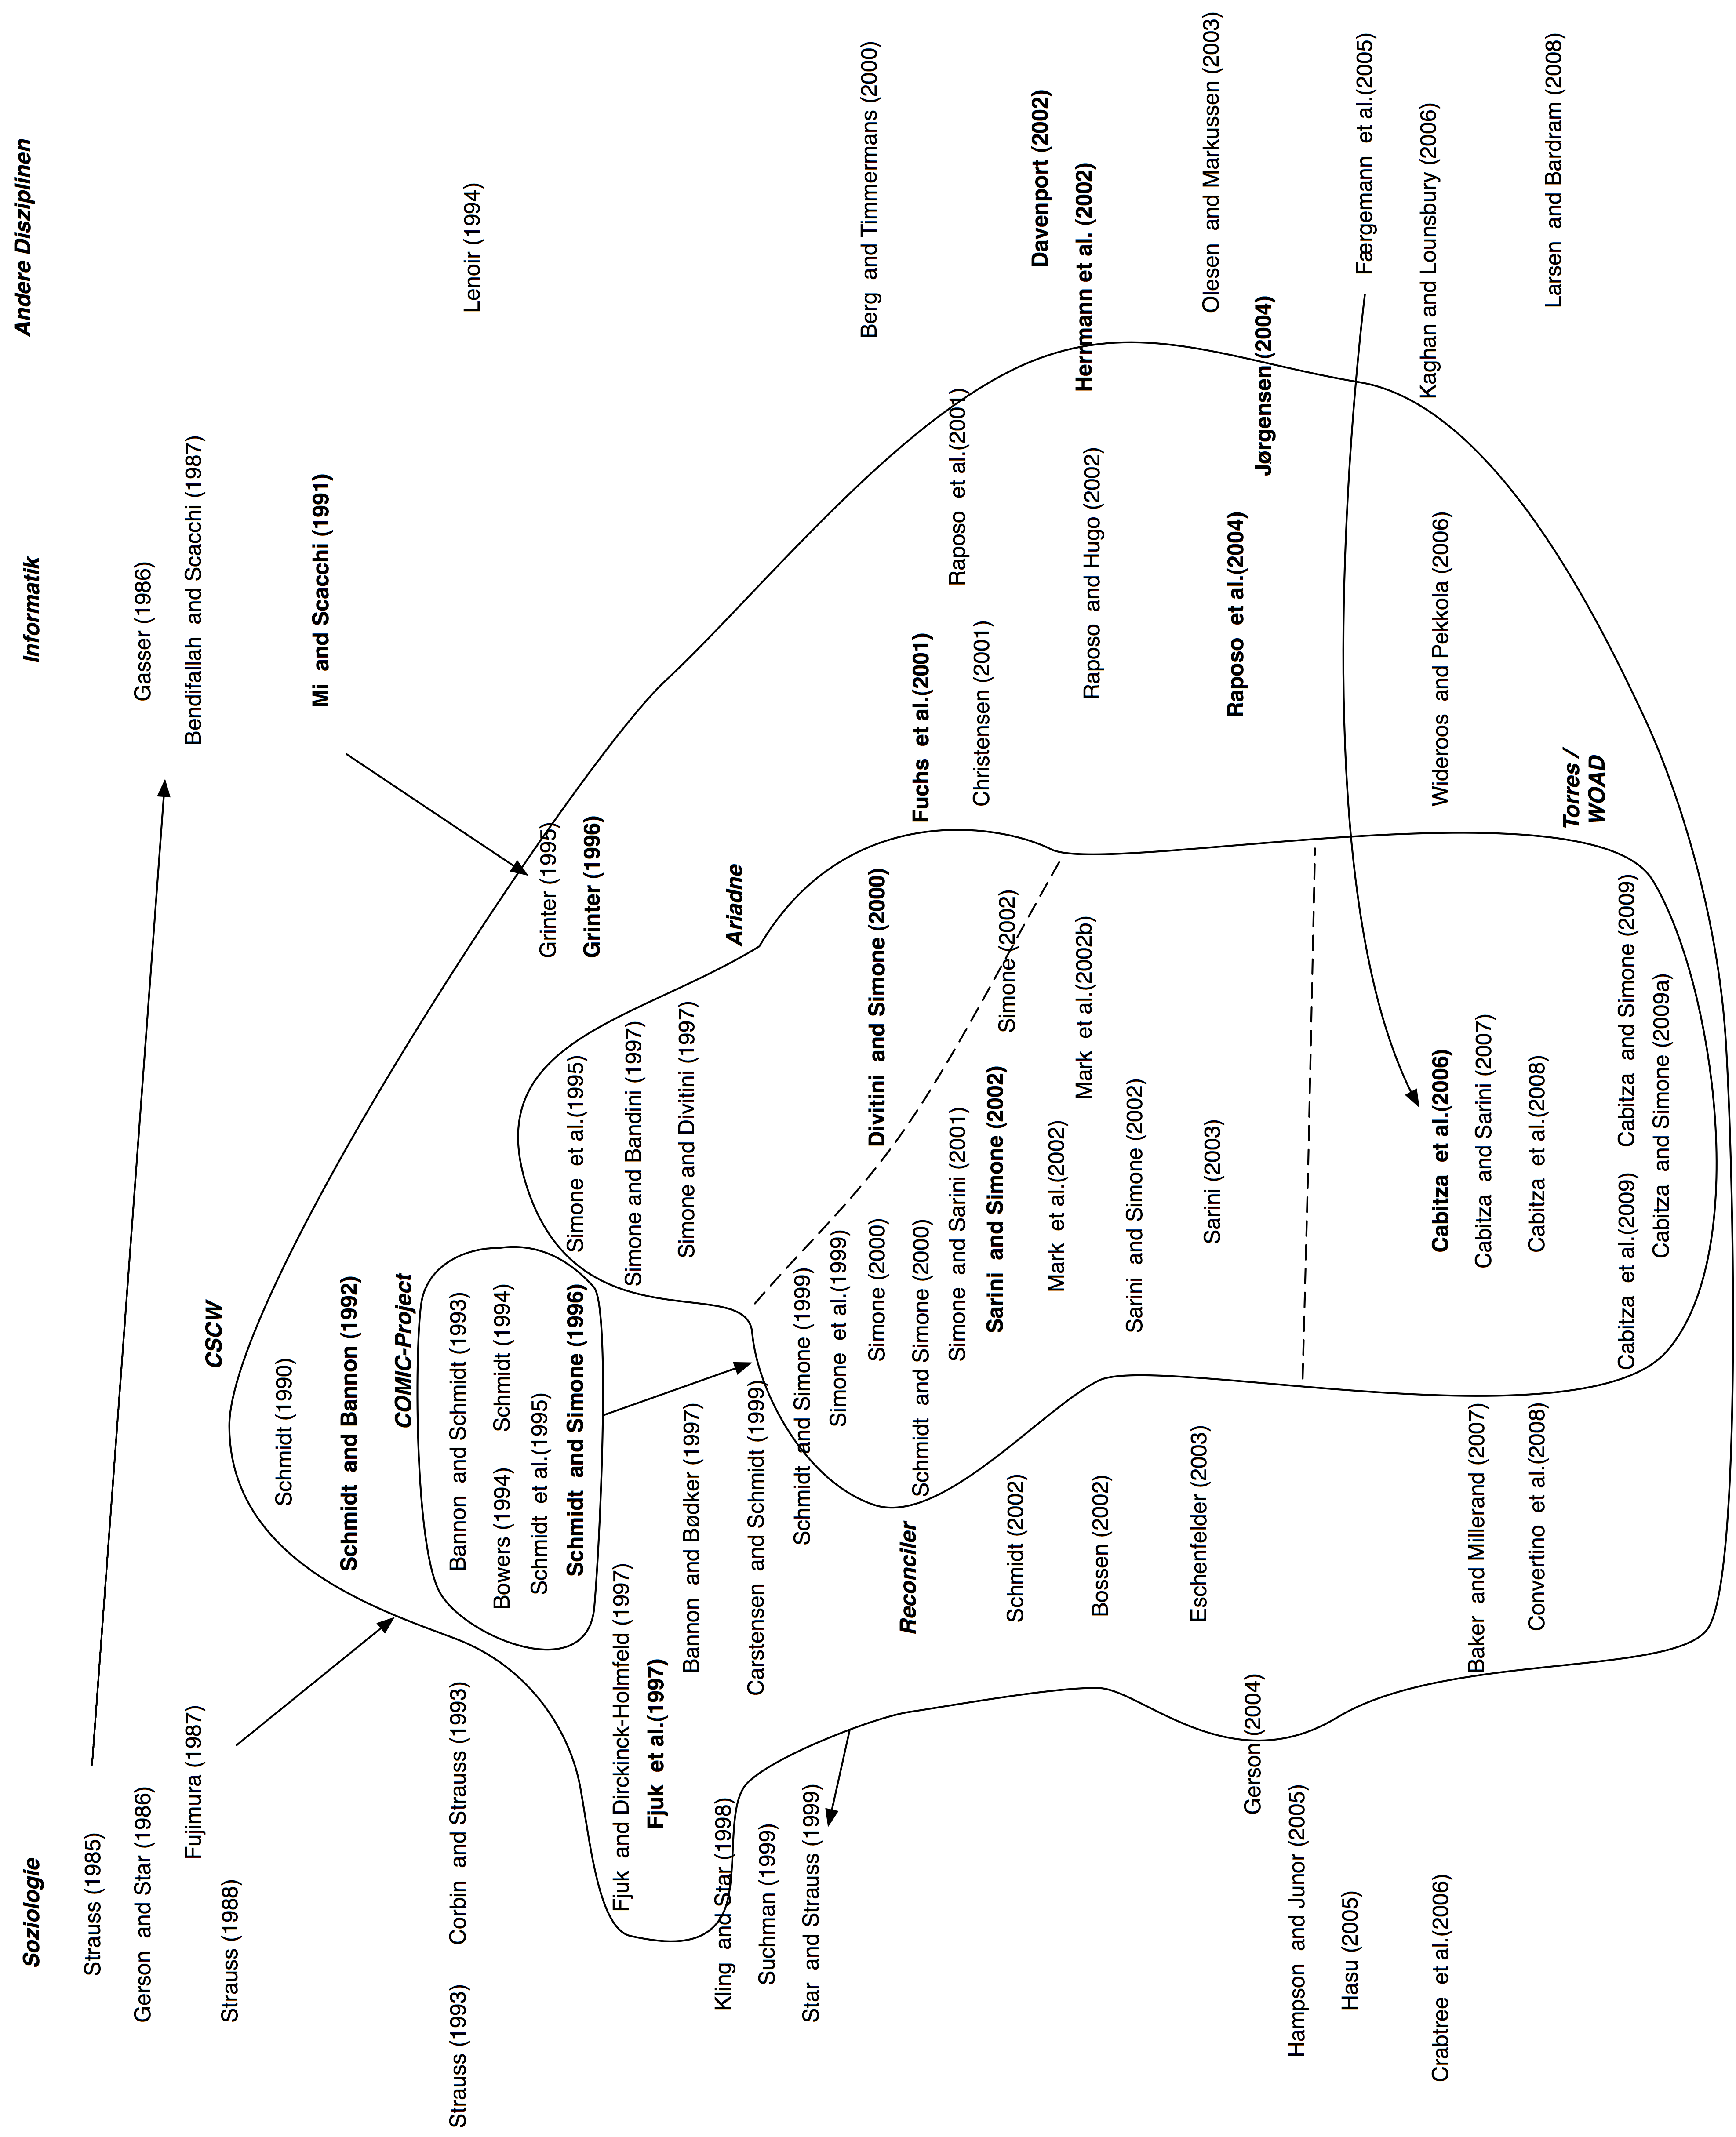
\includegraphics[width=\textwidth]{img/ArticulationWork/ArticulationWorkLiteratur.png}
	\caption{Literatur zu Articulation Work im Kontext}
	\label{fig:img_ArticulationWork_ArticulationWorkLiteratur}
\end{figure}

Beginnend mit den Arbeiten von Strauss in der linken oberen Ecke ist vertikal die zeitliche Dimension der Publikation von Arbeiten zu Artikulation Work aufgetragen. Die Seitenbreite wird zur thematischen Gruppierung der Publikationen verwendet. Die Pfeile zwischen Publikationen bzw. Publikationsgruppen stellen einen inhaltlichen Bezug dar. Die Publikationen am Endpunkt des Pfeils nehmen dabei Bezug auf jene, die sich am Ausgangspunkt des Pfeils befinden.

Am linken Rand der Darstellung sind die Arbeiten zu finden, die im soziologischen Kontext verfasst wurden. Die meisten der dort angesiedelten Publikationen sind Grundlagenarbeiten, die den Begriff „Articulation Work“ und dessen konzeptionellen Kontext erörtern oder anhand von Fallstudien das Auftreten von „Articulation Work“ zeigen.

Im Zentrum der Darstellung steht die größte Gruppe von Arbeiten, die im Kontext von \gls{CSCW} verfasst wurde. Die Arbeiten, die sich auf \gls{CSCW} beziehen, haben dabei zum Teil die Ableitung für Anforderungen an eine technische Unterstützung von „Articulation Work“ zum Ziel, der Rest der Arbeiten beschäftigt sich eher mit der technischen Umsetzung der Unterstützung. Jene Publikationen, die eher ersterer Gruppe zuzuordnen sind, sind eher links angeordnet, die technisch orientierten Publikationen befinden sich eher rechts. Die Entfernung zur Mittelachse hat dabei keine Aussagekraft sondern ist nur einer übersichtlichen Anordnung geschuldet. 

Innerhalb der \gls{CSCW}-Gruppe gibt es zwei bedeutende Sub-Gruppen, die untereinander in Beziehung stehen. Einerseits ist die Gruppe von Publikationen zu nennen, die im Rahmen des COMIC-Projektes 1992-1995 entstanden sind \citep{Rodden95}. In diesem Projekt wurde die Grundlage der Berücksichtigung von „Articulation Work“ als Thema von \gls{CSCW} gelegt. Bereits im Rahmen des COMIC-Projektes beginnend, publiziert die Gruppe um \citeauthor{Simone00} Arbeiten zur konkreten technischen Umsetzung der Unterstützung durch computerbasierte Werkzeuge. Die Implementierungen, auf die dabei immer wieder Bezug genommen wird, werden als „Ariadne“ (für den Koordinierungsaspekt von „Articulation Work“) „Reconciler“ (für den Awareness-Aspekt von „Articulation Work“) bezeichnet, was auch als Namensgeber dieser Gruppe von Arbeiten herangezogen wurde.

Weiter rechts am oberen Rand der Abbildung befinden sich Arbeiten, die Articulation Work im Kontext der Software-Entwicklung betrachten. Dies sind die ersten Arbeiten, die eine konkrete Anwendung der Konzepte um „Articulation Work“ außerhalb der Soziologie bzw. der Community um Strauss zeigen. Die Unterstützung von Articulation Work ist hier nur teilweise Gegenstand der Betrachtung, wo sie aber angesprochen wird ist sie entsprechend der Anwendungsdomäne eher technisch orientiert.

Ganz rechts sind jene Arbeiten zu finden, die auf „Articulation Work“ Bezug nehmen, jedoch nicht einer der bisher beschriebenen Gruppen zuzuordnen sind. Hier finden sich Publikationen die vor philosophischem, organsationswissenschaftlichem Hintergrund oder mit Bezug zum Wissensmanagement verfasst wurden. Herauszugreifen ist hier die Arbeit von \citet{Jorgensen04}, der die Rolle von Modellen (konkret konzeptionellen Modellen von Arbeit) bei der Durchführung von „Articulation Work“ betrachtet und damit erstmals einen konkreten Unterstützungsbezug zwischen „Artikulation Work“ und der Domäne der Organisationswissenschaften herstellt (was wiederum für die Betrachtung von „Articulation Work“ im organisationalen Kontext von Interesse ist).

Insgesamt ist in der Abbildung ein starker Schwerpunkt auf die technische Unterstützung von Arbeit, konkret „Articulation Work“, zu erkennen. Dieser Schwerpunkt wurde sowohl konzeptionell als auch technisch ab Beginn der 90er-Jahre des 20. Jahrhunderts bis etwa 2005 ausführlich bearbeitet. In den letzten Jahren treten verstärkt Fallstudien auf, die einen Bezug zu „Articulation Work“ herstellen, jedoch nur bedingt auf deren Unterstützung eingehen.

% section relevante_literatur (end)

% chapter literatur_zum_themengebiet_articulation_work (end)